% answers.tex —— 2009 年·普通高等学校招生考试·江苏卷 · 参考答案与详细解析片段
% 由 tools/generate_projects.py 依来源总账自 2009/2009_数学真题_江苏_试题.md + 2009/2009_数学真题_江苏_解析正文.md + 2009/2009_数学真题_江苏_答案要点.md 生成，勿手改（改源 MD 后重跑）


\begin{gktip}
固定候选 PDF 仅含题面，无答案、解析和评分标准，原页亦未标分值；以下为非官方编者独立推导，官方答案字段为空。题面文字层只作定位，分数、根号、上下标与七幅图均以 600 dpi 原页复核。原页第 18 题「互相垂的直线」、第 19 题 (1) 的「求 $h$ 和 $h_{\text{\text{乙}}}$」照录并在相应题目中说明；第 19 题原页未印 $m_A$、$m_B$ 的取值范围，已在解析中分别讨论并登记阻断项。
\end{gktip}

\begin{answer}
\gksolhead{1}{}

\textbf{题目}：

若复数 $z_1=4+29\mathrm i$，$z_2=6+9\mathrm i$，其中 $\mathrm i$ 是虚数单位，则复数 $(z_1-z_2)\mathrm i$ 的实部为\gkblank{}。

\Needspace{4\baselineskip}
\textbf{解析}

\Needspace{5\baselineskip}
先作差：

\nopagebreak[4]
\[z_1-z_2=(4+29\mathrm i)-(6+9\mathrm i)=-2+20\mathrm i .\]

\Needspace{5\baselineskip}
再乘 $\mathrm i$：

\nopagebreak[4]
\[(z_1-z_2)\mathrm i=(-2+20\mathrm i)\mathrm i=-20-2\mathrm i .\]

实部为 $-20$。

\gkanswer{答案：$-20$。}

\end{answer}
\begin{answer}
\gksolhead{2}{}

\textbf{题目}：

已知向量 $\boldsymbol a$ 和向量 $\boldsymbol b$ 的夹角为 $30^\circ$，$|\boldsymbol a|=2$，$|\boldsymbol b|=\sqrt3$，则向量 $\boldsymbol a$ 和向量 $\boldsymbol b$ 的数量积 $\boldsymbol a\cdot\boldsymbol b=$\gkblank{}。

\Needspace{4\baselineskip}
\textbf{解析}

\Needspace{5\baselineskip}
由数量积定义 $\boldsymbol a\cdot\boldsymbol b=|\boldsymbol a||\boldsymbol b|\cos\langle\boldsymbol a,\boldsymbol b\rangle$，代入得

\nopagebreak[4]
\[\boldsymbol a\cdot\boldsymbol b=2\times\sqrt3\times\cos30^\circ=2\sqrt3\times\frac{\sqrt3}2=3 .\]

\gkanswer{答案：$3$。}

\end{answer}
\begin{answer}
\gksolhead{3}{}

\textbf{题目}：

函数 $f(x)=x^3-15x^2-33x+6$ 的单调减区间为\gkblank{}。

\Needspace{4\baselineskip}
\textbf{解析}

\Needspace{5\baselineskip}
求导：

\nopagebreak[4]
\[f'(x)=3x^2-30x-33=3(x-11)(x+1) .\]

当 $-1<x<11$ 时 $f'(x)<0$，故 $f(x)$ 的单调减区间为 $(-1,11)$。

\gkanswer{答案：$(-1,11)$。}

\end{answer}
\begin{answer}
\gksolhead{4}{}

\textbf{题目}：

函数 $y=A\sin(\omega x+\varphi)$（$A$，$\omega$，$\varphi$ 为常数，$A>0$，$\omega>0$）在闭区间 $[-\pi,0]$ 上的图象如图所示，则 $\omega=$\gkblank{}。
\nopagebreak[4]
\begin{center}% 2009 年江苏卷第 4 题：y=A sin(ωx+φ) 在 [−π,0] 上的图象。
% 来源 PDF：普通高考/2009/2009江苏.pdf
% SHA-256：64e417d45911d88d77c047a419dcc259e7c7dc779c79d20df2092755c96a4501
% 原页：2009江苏.pdf 第 1 页（A3 三栏）第 1 栏，书页码 531。
% 绘制依据：按原页曲线在 [−π,0] 上与 x 轴依次交于 −π、−2π/3、−π/3、0，
%   在 −π/2 处取最大值，在 −5π/6、−π/6 处取最小值；取 A=1、φ=0 绘 y=sin3x。
\begin{tikzpicture}[x=1.15cm, y=1.15cm, semithick, every node/.style={inner sep=1.6pt}]
  \draw[->,>=stealth] (-3.55,0) -- (0.75,0) node[below] {$x$};
  \draw[->,>=stealth] (0,-1.55) -- (0,1.75) node[right] {$y$};

  \draw[domain=-3.14159:0, samples=160, smooth] plot (\x,{sin(3*\x r)});

  \node[below left] at (-3.14159,0) {$-\pi$};
  \node[above] at (-2.42,0.06) {$-\dfrac{2\pi}3$};
  \node[above] at (-0.70,0.06) {$-\dfrac{\pi}3$};
  \node[below right] at (0.06,-0.05) {$O$};
\end{tikzpicture}
\end{center}
\nopagebreak[4]
\Needspace{4\baselineskip}
\textbf{解析}

\Needspace{5\baselineskip}
图中曲线在 $[-\pi,0]$ 上与 $x$ 轴的交点依次为 $-\pi$、$-\dfrac{2\pi}3$、$-\dfrac{\pi}3$、$0$。相邻两个零点之间的距离为 $\dfrac{\pi}3$，等于半个周期，故

\nopagebreak[4]
\[T=2\times\frac{\pi}3=\frac{2\pi}3,\qquad \omega=\frac{2\pi}T=3 .\]

\gkanswer{答案：$3$。}

\end{answer}
\begin{answer}
\gksolhead{5}{}

\textbf{题目}：

现有 $5$ 根竹竿，它们的长度（单位：m）分别为 $2.5$，$2.6$，$2.7$，$2.8$，$2.9$，若从中一次随机抽取 $2$ 根竹竿，则它们的长度恰好相差 $0.3$ m 的概率为\gkblank{}。

\Needspace{4\baselineskip}
\textbf{解析}

\Needspace{5\baselineskip}
从 $5$ 根竹竿中一次抽取 $2$ 根，共有 $\mathrm C_5^2=10$ 种等可能的结果。长度恰好相差 $0.3$ m 的只有 $\{2.5,2.8\}$ 与 $\{2.6,2.9\}$ 两组，故所求概率为

\nopagebreak[4]
\[P=\frac2{10}=\frac15 .\]

\gkanswer{答案：$\dfrac15$。}

\end{answer}
\begin{answer}
\gksolhead{6}{}

\textbf{题目}：

某校甲、乙两个班级各有 $5$ 名编号为 $1$，$2$，$3$，$4$，$5$ 的学生进行投篮练习，每人投 $10$ 次，投中的次数如下表：

\begin{center}
\begin{tabular}{llllll}
\toprule
学生 & 1 号 & 2 号 & 3 号 & 4 号 & 5 号 \\
\midrule
甲班 & 6 & 7 & 7 & 8 & 7 \\
乙班 & 6 & 7 & 6 & 7 & 9 \\
\bottomrule
\end{tabular}
\end{center}

则以上两组数据的方差中较小的一个为 $s^2=$\gkblank{}。

\Needspace{4\baselineskip}
\textbf{解析}

\Needspace{5\baselineskip}
甲班 $5$ 个数据 $6,7,7,8,7$ 的平均数为 $7$，方差

\nopagebreak[4]
\[s_{\text{\text{甲}}}^2=\frac{(6-7)^2+0+0+(8-7)^2+0}5=\frac25 .\]

\Needspace{5\baselineskip}
乙班 $5$ 个数据 $6,7,6,7,9$ 的平均数为 $7$，方差

\nopagebreak[4]
\[s_{\text{\text{乙}}}^2=\frac{(6-7)^2+0+(6-7)^2+0+(9-7)^2}5=\frac65 .\]

较小的一个为 $\dfrac25$。

\gkanswer{答案：$\dfrac25$。}

\end{answer}
\begin{answer}
\gksolhead{7}{}

\textbf{题目}：

如图是一个算法的流程图，最后输出的 $W=$\gkblank{}。
\nopagebreak[4]
\begin{center}% 2009 年江苏卷第 7 题：求 W 的算法流程图。
% 来源 PDF：普通高考/2009/2009江苏.pdf
% SHA-256：64e417d45911d88d77c047a419dcc259e7c7dc779c79d20df2092755c96a4501
% 原页：2009江苏.pdf 第 1 页（A3 三栏）第 1 栏，书页码 531。
% 绘制依据：按原页流程：开始 → S←0 → T←1 → S←T²−S → 判断 S≥10 →
%   N 时 T←T+2 回环 → Y 时 W←S+T → 输出 W → 结束。
\begin{tikzpicture}[node distance=0.55cm, semithick, every node/.style={inner sep=3pt},
  box/.style={draw, minimum width=2.0cm, minimum height=0.55cm},
  io/.style={draw, trapezium, trapezium left angle=70, trapezium right angle=110,
             minimum width=2.3cm, minimum height=0.55cm},
  dec/.style={draw, diamond, aspect=1.9, inner sep=1pt}]

  \node[box, rounded corners=2pt] (start) {开始};
  \node[box, below=of start] (s0) {$S\leftarrow0$};
  \node[box, below=of s0] (t1) {$T\leftarrow1$};
  \node[dec, below=0.6cm of t1, minimum width=2.4cm, minimum height=0.95cm] (assign)
    {$S\leftarrow T^2-S$};
  \node[dec, below=0.55cm of assign, minimum width=1.9cm, minimum height=0.95cm] (test)
    {$S\geqslant10$};
  \node[box, below=0.65cm of test] (w) {$W\leftarrow S+T$};
  \node[io, below=of w] (out) {输出 $W$};
  \node[box, rounded corners=2pt, below=of out] (end) {结束};
  \node[box, right=1.5cm of assign] (inc) {$T\leftarrow T+2$};

  \draw[->,>=stealth] (start) -- (s0);
  \draw[->,>=stealth] (s0) -- (t1);
  \draw[->,>=stealth] (t1) -- (assign);
  \draw[->,>=stealth] (assign) -- (test);
  \draw[->,>=stealth] (test) -- node[left] {Y} (w);
  \draw[->,>=stealth] (w) -- (out);
  \draw[->,>=stealth] (out) -- (end);
  \draw[->,>=stealth] (test.east) -- node[above] {N} ++(0.30,0) -| (inc.south);
  \draw (inc.north) -- ++(0,0.65) -| ($(t1.south)!0.45!(assign.north)$);
\end{tikzpicture}
\end{center}
\nopagebreak[4]
\Needspace{4\baselineskip}
\textbf{解析}

按流程图逐步执行：

\begin{itemize}
\item $S=0$，$T=1$；
\item $S=1^2-0=1$，因 $1<10$，$T=1+2=3$；
\item $S=3^2-1=8$，因 $8<10$，$T=3+2=5$；
\item $S=5^2-8=17$，因 $17\geqslant10$，退出循环，$W=17+5=22$。
\end{itemize}

输出的 $W=22$。

\gkanswer{答案：$22$。}

\end{answer}
\begin{answer}
\gksolhead{8}{}

\textbf{题目}：

在平面上，若两个正三角形的边长的比为 $1:2$，则它们的面积比为 $1:4$，类似地，在空间内，若两个正四面体的棱长的比为 $1:2$，则它们的体积比为\gkblank{}。

\Needspace{4\baselineskip}
\textbf{解析}

\Needspace{5\baselineskip}
两个正三角形的边长比为 $1:2$ 时面积比为 $1^2:2^2=1:4$，这是平面图形「面积比等于相似比的平方」。类比到空间，两个正四面体相似，体积比等于相似比的立方，故体积比为

\nopagebreak[4]
\[1^3:2^3=1:8 .\]

\gkanswer{答案：$1:8$。}

\end{answer}
\begin{answer}
\gksolhead{9}{}

\textbf{题目}：

在平面直角坐标系 $xOy$ 中，点 $P$ 在曲线 $C$：$y=x^3-10x+3$ 上，且在第二象限内，已知曲线 $C$ 在点 $P$ 处的切线的斜率为 $2$，则点 $P$ 的坐标为\gkblank{}。

\Needspace{4\baselineskip}
\textbf{解析}

\Needspace{5\baselineskip}
由 $y=x^3-10x+3$ 得 $y'=3x^2-10$。令 $3x^2-10=2$，得 $x^2=4$，$x=\pm2$。点 $P$ 在第二象限，故 $x=-2$，此时

\nopagebreak[4]
\[y=(-2)^3-10\times(-2)+3=15 .\]

故 $P(-2,15)$。

\gkanswer{答案：$(-2,15)$。}

\end{answer}
\begin{answer}
\gksolhead{10}{}

\textbf{题目}：

已知 $a=\dfrac{\sqrt5-1}{2}$，函数 $f(x)=a^x$，若实数 $m$、$n$ 满足 $f(m)>f(n)$，则 $m$、$n$ 的大小关系为\gkblank{}。

\Needspace{4\baselineskip}
\textbf{解析}

因为 $1<\sqrt5<3$，所以 $0<\dfrac{\sqrt5-1}2<1$。于是 $f(x)=a^x$ 在 $\mathbf R$ 上单调递减，$f(m)>f(n)$ 等价于 $m<n$。

\gkanswer{答案：$m<n$。}

\end{answer}
\begin{answer}
\gksolhead{11}{}

\textbf{题目}：

已知集合 $A=\{x\mid \log_2x\leqslant2\}$，$B=(-\infty,a)$，若 $A\subseteq B$，则实数 $a$ 的取值范围是 $(c,+\infty)$，其中 $c=$\gkblank{}。

\Needspace{4\baselineskip}
\textbf{解析}

由 $\log_2x\leqslant2=\log_24$ 且对数定义域为 $x>0$，得 $A=(0,4]$。

$A\subseteq B=(-\infty,a)$ 要求 $(0,4]$ 中每个数都小于 $a$，即 $a>4$（$a=4$ 时 $4\notin B$）。对照题设「$a$ 的取值范围是 $(c,+\infty)$」，得 $c=4$。

\gkanswer{答案：$4$。}

\end{answer}
\begin{answer}
\gksolhead{12}{}

\textbf{题目}：

设 $\alpha$ 和 $\beta$ 为不重合的两个平面，给出下列命题：

（1）若 $\alpha$ 内的两条相交直线分别平行于 $\beta$ 内的两条直线，则 $\alpha$ 平行于 $\beta$；

（2）若 $\alpha$ 外一条直线 $l$ 与 $\alpha$ 内的一条直线平行，则 $l$ 和 $\alpha$ 平行；

（3）设 $\alpha$ 和 $\beta$ 相交于直线 $l$，若 $\alpha$ 内有一条直线垂直于 $l$，则 $\alpha$ 和 $\beta$ 垂直；

（4）直线 $l$ 与 $\alpha$ 垂直的充分必要条件是 $l$ 与 $\alpha$ 内的两条直线垂直。

上面命题中，真命题的序号\gkblank{}。（写出所有真命题的序号）

\Needspace{4\baselineskip}
\textbf{解析}

（1）$\alpha$ 内两条相交直线确定平面 $\alpha$；它们分别平行于 $\beta$ 内的两条直线，由平行传递性，$\beta$ 内这两条直线也相交，且都平行于 $\alpha$，由面面平行的判定定理得 $\alpha\parallel\beta$。真。

（2）$l$ 在 $\alpha$ 外，且与 $\alpha$ 内一条直线平行，由线面平行的判定定理得 $l\parallel\alpha$。真。

（3）$\alpha$ 内垂直于交线 $l$ 的直线只保证与 $l$ 垂直，不一定垂直于 $\beta$（还需垂直于 $\beta$ 内另一条相交直线）。假。

（4）判定线面垂直需要 $l$ 垂直于平面内两条\textbf{相交}直线，仅「两条直线」不够。假。

故真命题的序号为（1）（2）。

\gkanswer{答案：（1）（2）。}

\end{answer}
\begin{answer}
\gksolhead{13}{}

\textbf{题目}：

如图，在平面直角坐标系 $xOy$ 中，$A_1$，$A_2$，$B_1$，$B_2$ 为椭圆 $\dfrac{x^2}{a^2}+\dfrac{y^2}{b^2}=1$（$a>b>0$）的四个顶点，$F$ 为其右焦点，直线 $A_1B_2$ 与直线 $B_1F$ 相交于点 $T$，线段 $OT$ 与椭圆的交点 $M$ 恰为线段 $OT$ 的中点，则该椭圆的离心率为\gkblank{}。
\nopagebreak[4]
\begin{center}% 2009 年江苏卷第 13 题：椭圆的四个顶点、右焦点 F、交点 T 与中点 M。
% 来源 PDF：普通高考/2009/2009江苏.pdf
% SHA-256：64e417d45911d88d77c047a419dcc259e7c7dc779c79d20df2092755c96a4501
% 原页：2009江苏.pdf 第 1 页（A3 三栏）第 2 栏，书页码 531。
% 绘制依据：按原页画椭圆 A1A2B2B1、右焦点 F、直线 A1B2 与 B1F 的交点 T，
%   以及 OT 的中点 M（落在椭圆上）；示意取 a=2.6，b≈2.487，e=2√7−5。
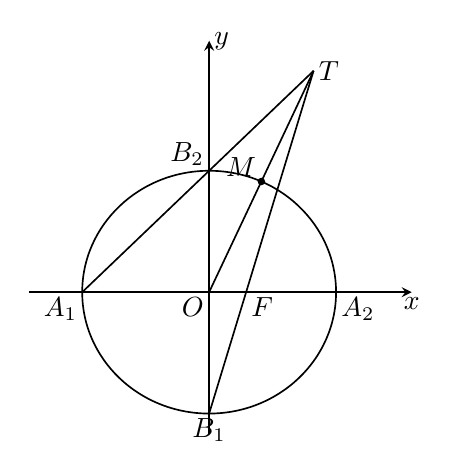
\begin{tikzpicture}[scale=0.62, semithick, every node/.style={inner sep=1.6pt}]
  \draw (0,0) ellipse [x radius=2.6, y radius=2.4868];

  \coordinate (A1) at (-2.6,0);
  \coordinate (A2) at (2.6,0);
  \coordinate (B1) at (0,-2.4868);
  \coordinate (B2) at (0,2.4868);
  \coordinate (F) at (0.7579,0);
  \coordinate (T) at (2.1394,4.5335);
  \coordinate (M) at (1.0697,2.2668);

  \draw[->,>=stealth] (-3.7,0) -- (4.15,0) node[below] {$x$};
  \draw[->,>=stealth] (0,-2.9) -- (0,5.15) node[right] {$y$};

  \draw (A1) -- (T);
  \draw (B1) -- (T);
  \draw (0,0) -- (T);

  \fill (M) circle (2.2pt);

  \node[below left] at (A1) {$A_1$};
  \node[below right] at (A2) {$A_2$};
  \node[below] at (B1) {$B_1$};
  \node[above left] at (B2) {$B_2$};
  \node[below right] at (F) {$F$};
  \node[right] at (T) {$T$};
  \node[above left] at (M) {$M$};
  \node[below left] at (0,0) {$O$};
\end{tikzpicture}
\end{center}
\nopagebreak[4]
\Needspace{4\baselineskip}
\textbf{解析}

设 $A_1(-a,0)$，$A_2(a,0)$，$B_1(0,-b)$，$B_2(0,b)$，$F(c,0)$。

直线 $A_1B_2$ 的方程为 $\dfrac x{-a}+\dfrac yb=1$，即 $y=\dfrac ba(x+a)$；直线 $B_1F$ 的方程为 $\dfrac xc-\dfrac yb=1$，即 $y=\dfrac bcx-b$。

\Needspace{5\baselineskip}
联立：

\nopagebreak[4]
\[\frac ba(x+a)=\frac bcx-b\ \Longrightarrow\ 2=\frac{x(a-c)}{ac}\ \Longrightarrow\ x_T=\frac{2ac}{a-c},\]

\nopagebreak[4]
\[y_T=\frac ba\left(\frac{2ac}{a-c}+a\right)=\frac{b(a+c)}{a-c}.\]

\Needspace{5\baselineskip}
$M$ 为 $OT$ 的中点，故

\nopagebreak[4]
\[M\left(\frac{ac}{a-c},\ \frac{b(a+c)}{2(a-c)}\right).\]

\Needspace{5\baselineskip}
代入椭圆方程：

\nopagebreak[4]
\[\frac{c^2}{(a-c)^2}+\frac{(a+c)^2}{4(a-c)^2}=1 .\]

\Needspace{5\baselineskip}
两边乘 $4(a-c)^2$：

\nopagebreak[4]
\[4c^2+(a+c)^2=4(a-c)^2\ \Longrightarrow\ c^2+10ac-3a^2=0 .\]

\Needspace{5\baselineskip}
两边除以 $a^2$，令 $e=\dfrac ca$，得 $e^2+10e-3=0$，解得 $e=-5\pm2\sqrt7$。由 $0<e<1$ 得

\nopagebreak[4]
\[e=2\sqrt7-5 .\]

\gkanswer{答案：$2\sqrt7-5$。}

\end{answer}
\begin{answer}
\gksolhead{14}{}

\textbf{题目}：

设 $\{a_n\}$ 是公比为 $q$ 的等比数列，$|q|>1$，令 $b_n=a_n+1$（$n=1,2,\cdots$），若数列 $\{b_n\}$ 有连续四项在集合 $\{-53,-23,19,37,82\}$ 中，则 $6q=$\gkblank{}。

\Needspace{4\baselineskip}
\textbf{解析}

\Needspace{5\baselineskip}
由 $b_n=a_n+1$ 得 $a_n=b_n-1$，故 $\{a_n\}$ 中有连续四项属于

\nopagebreak[4]
\[\{-54,-24,18,36,81\}.\]

\Needspace{5\baselineskip}
按 $|q|>1$ 逐组检验相邻两项之比，只有

\nopagebreak[4]
\[-24,\ 36,\ -54,\ 81\]

满足公比相同：$36\div(-24)=-\dfrac32$，$(-54)\div36=-\dfrac32$，$81\div(-54)=-\dfrac32$。故 $q=-\dfrac32$，$6q=-9$。

\gkanswer{答案：$-9$。}

\end{answer}
\begin{answer}
\gksolhead{15}{}

\textbf{题目}：

设向量 $\boldsymbol a=(4\cos\alpha,\sin\alpha)$，$\boldsymbol b=(\sin\beta,4\cos\beta)$，$\boldsymbol c=(\cos\beta,-4\sin\beta)$。

（1）若 $\boldsymbol a$ 与 $\boldsymbol b-2\boldsymbol c$ 垂直，求 $\tan(\alpha+\beta)$ 的值；

（2）求 $|\boldsymbol b+\boldsymbol c|$ 的最大值；

（3）若 $\tan\alpha\tan\beta=16$，求证：$\boldsymbol a\parallel\boldsymbol b$。

\Needspace{4\baselineskip}
\textbf{解析}

\Needspace{5\baselineskip}
（1）先算 $\boldsymbol b-2\boldsymbol c$：

\nopagebreak[4]
\[\boldsymbol b-2\boldsymbol c=(\sin\beta-2\cos\beta,\ 4\cos\beta+8\sin\beta).\]

\Needspace{5\baselineskip}
由 $\boldsymbol a\perp(\boldsymbol b-2\boldsymbol c)$ 得

\nopagebreak[4]
\[4\cos\alpha(\sin\beta-2\cos\beta)+\sin\alpha(4\cos\beta+8\sin\beta)=0 .\]

\Needspace{5\baselineskip}
两边除以 $4$，按 $\sin(\alpha+\beta)$、$\cos(\alpha+\beta)$ 合并：

\nopagebreak[4]
\[\begin{aligned}
&\cos\alpha\sin\beta+\sin\alpha\cos\beta-2(\cos\alpha\cos\beta-\sin\alpha\sin\beta)\\
&=\sin(\alpha+\beta)-2\cos(\alpha+\beta)=0 .
\end{aligned}\]

\Needspace{5\baselineskip}
若 $\cos(\alpha+\beta)=0$，则 $\sin(\alpha+\beta)=0$，矛盾，故 $\cos(\alpha+\beta)\neq0$，从而

\nopagebreak[4]
\[\tan(\alpha+\beta)=2 .\]

\Needspace{5\baselineskip}
（2）由 $\boldsymbol b+\boldsymbol c=(\sin\beta+\cos\beta,\ 4\cos\beta-4\sin\beta)$ 得

\nopagebreak[4]
\[|\boldsymbol b+\boldsymbol c|^2=(1+\sin2\beta)+16(1-\sin2\beta)=17-15\sin2\beta .\]

因为 $-1\leqslant\sin2\beta\leqslant1$，所以 $|\boldsymbol b+\boldsymbol c|^2\leqslant32$，当 $\sin2\beta=-1$ 时取等号，最大值为 $\sqrt{32}=4\sqrt2$。

\Needspace{5\baselineskip}
（3）$\boldsymbol a\parallel\boldsymbol b$ 等价于

\nopagebreak[4]
\[4\cos\alpha\cdot4\cos\beta-\sin\alpha\cdot\sin\beta=0 .\]

\Needspace{5\baselineskip}
由 $\tan\alpha\tan\beta=16>0$ 知 $\cos\alpha\cos\beta\neq0$，上式两边同除以 $\cos\alpha\cos\beta$ 得

\nopagebreak[4]
\[16-\tan\alpha\tan\beta=0,\]

即 $\tan\alpha\tan\beta=16$，恰为已知条件，故 $\boldsymbol a\parallel\boldsymbol b$。

\gkanswer{答案：（1）$2$；（2）$4\sqrt2$；（3）证明见解析。}

\end{answer}
\begin{answer}
\gksolhead{16}{}

\textbf{题目}：

如图，在直三棱柱 $ABC-A_1B_1C_1$ 中，$E$、$F$ 分别是 $A_1B$、$A_1C$ 的中点，点 $D$ 在 $B_1C_1$ 上，$A_1D\perp B_1C$。求证：

（1）$EF\parallel$ 平面 $ABC$；

（2）平面 $A_1FD\perp$ 平面 $BB_1C_1C$。
\nopagebreak[4]
\begin{center}% 2009 年江苏卷第 16 题：直三棱柱 ABC−A1B1C1，E、F 为 A1B、A1C 中点，D 在 B1C1 上。
% 来源 PDF：普通高考/2009/2009江苏.pdf
% SHA-256：64e417d45911d88d77c047a419dcc259e7c7dc779c79d20df2092755c96a4501
% 原页：2009江苏.pdf 第 1 页（A3 三栏）第 3 栏，书页码 531。
% 绘制依据：按原页斜投影；被遮挡的 AC 与 A1B1 用虚线，其余实线；
%   E 在 A1B 上、F 在 A1C 上，D 在 B1C1 上，A1D 连实线。
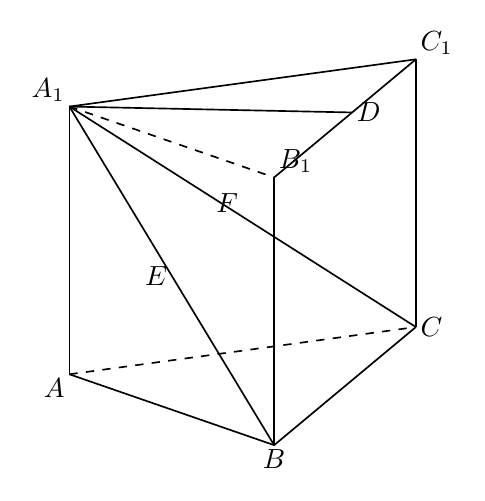
\begin{tikzpicture}[scale=1.0, semithick, every node/.style={inner sep=1.4pt}]
  \coordinate (A) at (0,0);
  \coordinate (A1) at (0,3.4);
  \coordinate (B) at (2.6,-0.9);
  \coordinate (B1) at (2.6,2.5);
  \coordinate (C) at (4.4,0.6);
  \coordinate (C1) at (4.4,4.0);
  \coordinate (D) at (3.59,3.325);
  \coordinate (E) at (1.3,1.25);
  \coordinate (F) at (2.2,2.0);

  % 前面与可见棱
  \draw (A) -- (B) -- (C);
  \draw (A) -- (A1);
  \draw (B) -- (B1);
  \draw (C) -- (C1);
  \draw (A1) -- (C1);
  \draw (B1) -- (C1);
  % 面内连线
  \draw (A1) -- (B);
  \draw (A1) -- (C);
  \draw (A1) -- (D);

  % 被遮挡的棱
  \draw[dashed] (A) -- (C);
  \draw[dashed] (A1) -- (B1);

  \node[above left] at (A1) {$A_1$};
  \node[above right] at (C1) {$C_1$};
  \node[above right] at (B1) {$B_1$};
  \node[right] at (D) {$D$};
  \node[left] at (E) {$E$};
  \node[above left] at (F) {$F$};
  \node[below left] at (A) {$A$};
  \node[right] at (C) {$C$};
  \node[below] at (B) {$B$};
\end{tikzpicture}
\end{center}
\nopagebreak[4]
\Needspace{4\baselineskip}
\textbf{解析}

\Needspace{5\baselineskip}
（1）在 $\triangle A_1BC$ 中，$E$、$F$ 分别是 $A_1B$、$A_1C$ 的中点，故 $EF$ 为中位线，

\nopagebreak[4]
\[EF\parallel BC .\]

\Needspace{5\baselineskip}
又 $BC\subset$ 平面 $ABC$，而 $EF\not\subset$ 平面 $ABC$，由线面平行的判定定理得

\nopagebreak[4]
\[EF\parallel\text{\text{平面} }ABC .\]

（2）在直三棱柱 $ABC-A_1B_1C_1$ 中，侧棱 $CC_1\perp$ 平面 $A_1B_1C_1$，而 $A_1D\subset$ 平面 $A_1B_1C_1$，故 $CC_1\perp A_1D$。

又已知 $A_1D\perp B_1C$。$B_1C$ 与 $CC_1$ 是平面 $BB_1C_1C$ 内两条相交直线，故 $A_1D\perp\text{\text{平面} }BB_1C_1C$。

\Needspace{5\baselineskip}
而 $A_1D\subset$ 平面 $A_1FD$，所以

\nopagebreak[4]
\[\text{\text{平面} }A_1FD\perp\text{\text{平面} }BB_1C_1C .\]

\gkanswer{答案：（1）（2）证明见解析。}

\end{answer}
\begin{answer}
\gksolhead{17}{}

\textbf{题目}：

设 $\{a_n\}$ 是公差不为零的等差数列，$S_n$ 为其前 $n$ 项和，满足 $a_2^2+a_3^2=a_4^2+a_5^2$，$S_7=7$。

（1）求数列 $\{a_n\}$ 的通项公式及前 $n$ 项和 $S_n$；

（2）试求所有的正整数 $m$，使得 $\dfrac{a_ma_{m+1}}{a_{m+2}}$ 为数列 $\{a_n\}$ 中的项。

\Needspace{4\baselineskip}
\textbf{解析}

\Needspace{5\baselineskip}
（1）设首项为 $a_1$，公差为 $d\neq0$，则 $a_2=a_1+d$，$a_3=a_1+2d$，$a_4=a_1+3d$，$a_5=a_1+4d$。由条件

\nopagebreak[4]
\[(a_1+d)^2+(a_1+2d)^2=(a_1+3d)^2+(a_1+4d)^2 .\]

\Needspace{5\baselineskip}
左边 $=2a_1^2+6a_1d+5d^2$，右边 $=2a_1^2+14a_1d+25d^2$，相减得

\nopagebreak[4]
\[8a_1d+20d^2=0 .\]

\Needspace{5\baselineskip}
因 $d\neq0$，故 $a_1=-\dfrac52d$。再由

\nopagebreak[4]
\[S_7=7a_1+\frac{7\times6}2d=7a_1+21d=7,\]

\Needspace{5\baselineskip}
即 $a_1+3d=1$。代入 $a_1=-\dfrac52d$ 得 $\dfrac d2=1$，故 $d=2$，$a_1=-5$。于是

\nopagebreak[4]
\[a_n=-5+2(n-1)=2n-7,\]

\nopagebreak[4]
\[S_n=\frac{n(a_1+a_n)}2=\frac{n(-5+2n-7)}2=n^2-6n .\]

\Needspace{5\baselineskip}
（2）令 $k=2m-3$，则 $k$ 为奇数，且 $2m-7=k-4$，$2m-5=k-2$，于是

\nopagebreak[4]
\[\frac{a_ma_{m+1}}{a_{m+2}}=\frac{(k-4)(k-2)}k=k-6+\frac8k .\]

若该式为 $\{a_n\}$ 中的项，则它必为奇数（$\{a_n\}$ 各项均为奇数），故 $\dfrac8k$ 为整数，$k\mid8$。又 $k$ 为奇数，故 $k=\pm1$。

当 $k=1$ 时 $m=2$，式值为 $1-6+8=3=a_5$，符合；

当 $k=-1$ 时 $m=1$，式值为 $-1-6-8=-15$，而 $a_n=2n-7\geqslant-5$，故 $-15\notin\{a_n\}$。

所以满足条件的正整数只有 $m=2$。

\gkanswer{答案：（1）$a_n=2n-7$，$S_n=n^2-6n$；（2）$m=2$。}

\end{answer}
\begin{answer}
\gksolhead{18}{}

\textbf{题目}：

在平面直角坐标系 $xOy$ 中，已知圆 $C_1$ 的方程为 $(x+3)^2+(y-1)^2=4$，圆 $C_2$ 的方程为 $(x-4)^2+(y-5)^2=4$。

（1）若直线 $l$ 过点 $A(4,0)$，且被圆 $C_1$ 截得的弦长为 $2\sqrt3$，求直线 $l$ 的方程；

（2）设 $P$ 为平面上的点，满足：存在过点 $P$ 的无穷多对互相垂的直线 $l_1$ 和 $l_2$，它们分别与圆 $C_1$ 和圆 $C_2$ 相交，且直线 $l_1$ 被圆 $C_1$ 截得的弦长与直线 $l_2$ 被圆 $C_2$ 截得的弦长相等，试求所有满足条件的点 $P$ 的坐标。
\nopagebreak[4]
\begin{center}% 2009 年江苏卷第 18 题：圆 C1:(x+3)²+(y−1)²=4 与圆 C2:(x−4)²+(y−5)²=4。
% 来源 PDF：普通高考/2009/2009江苏.pdf
% SHA-256：64e417d45911d88d77c047a419dcc259e7c7dc779c79d20df2092755c96a4501
% 原页：2009江苏.pdf 第 1 页（A3 三栏）第 3 栏，书页码 531。
% 绘制依据：按原页坐标画两圆（半径均为 2）、坐标轴、圆心与点 A(4,0)。
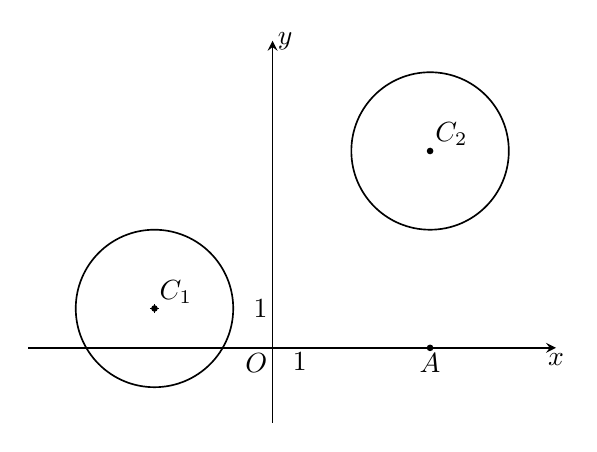
\begin{tikzpicture}[scale=0.5, semithick, every node/.style={inner sep=1.6pt}]
  \draw[->,>=stealth] (-6.2,0) -- (7.2,0) node[below] {$x$};
  \draw[->,>=stealth] (0,-1.9) -- (0,7.8) node[right] {$y$};

  \draw (-3,1) circle [radius=2];
  \draw (4,5) circle [radius=2];

  \fill (-3,1) circle (2.4pt);
  \fill (4,5) circle (2.4pt);
  \fill (4,0) circle (2.4pt);

  \draw (-3,1) ++(-0.12,0) -- ++(0.24,0);
  \draw (-3,1) ++(0,-0.12) -- ++(0,0.24);

  \node[above right] at (-3,1) {$C_1$};
  \node[above right] at (4,5) {$C_2$};
  \node[below] at (4,0) {$A$};
  \node[below left] at (0,0) {$O$};
  \node[below left] at (1,0) {$1$};
  \node[left] at (0,1) {$1$};
\end{tikzpicture}
\end{center}
\nopagebreak[4]
\Needspace{4\baselineskip}
\textbf{解析}

\Needspace{5\baselineskip}
（1）圆 $C_1$ 的圆心为 $O_1(-3,1)$，半径 $r=2$。弦长为 $2\sqrt3$，故圆心到直线 $l$ 的距离为

\nopagebreak[4]
\[d=\sqrt{r^2-\left(\frac{2\sqrt3}2\right)^2}=\sqrt{4-3}=1 .\]

若 $l$ 的斜率不存在，则 $l:x=4$，$O_1$ 到它的距离为 $7\neq1$，不合。

\Needspace{5\baselineskip}
设 $l:y=k(x-4)$，即 $kx-y-4k=0$，则

\nopagebreak[4]
\[\frac{|-3k-1-4k|}{\sqrt{k^2+1}}=1\ \Longrightarrow\ (7k+1)^2=k^2+1 .\]

展开得 $48k^2+14k=0$，即 $2k(24k+7)=0$，故 $k=0$ 或 $k=-\dfrac7{24}$。

\Needspace{5\baselineskip}
对应的直线为

\nopagebreak[4]
\[y=0\quad\text{\text{或}}\quad y=-\frac7{24}(x-4),\]

后者即 $7x+24y-28=0$。

（2）设 $P(x_0,y_0)$。取 $l_1$ 的单位方向向量为 $(\cos\theta,\sin\theta)$，与 $l_1$ 垂直的 $l_2$ 的方向向量可取 $(-\sin\theta,\cos\theta)$。

\Needspace{5\baselineskip}
两圆半径都是 $2$，故弦长相等等价于 $O_1$ 到 $l_1$ 的距离等于 $O_2$ 到 $l_2$ 的距离：

\nopagebreak[4]
\[|(-3-x_0)\sin\theta-(1-y_0)\cos\theta|=|(4-x_0)\cos\theta+(5-y_0)\sin\theta| .\]

\Needspace{5\baselineskip}
记 $A=-3-x_0$，$B=1-y_0$，$C=4-x_0$，$D=5-y_0$。要让上式对无穷多个 $\theta$ 成立，两边平方后 $\sin^2\theta$、$\cos^2\theta$、$\sin\theta\cos\theta$ 的系数必须分别相等：

\nopagebreak[4]
\[A^2=D^2,\qquad B^2=C^2,\qquad -2AB=2CD .\]

情形一：$A=D$，$B=-C$。由 $A=D$ 得 $y_0=x_0+8$，由 $B=-C$ 得 $y_0=5-x_0$，联立得 $x_0=-\dfrac32$，$y_0=\dfrac{13}2$。

情形二：$A=-D$，$B=C$。由 $A=-D$ 得 $y_0=2-x_0$，由 $B=C$ 得 $y_0=x_0-3$，联立得 $x_0=\dfrac52$，$y_0=-\dfrac12$。

两点到 $O_1$、$O_2$ 的距离都是 $\sqrt{\left(\dfrac32\right)^2+\left(\dfrac{11}2\right)^2}=\dfrac{\sqrt{130}}2>2$，故过每一点都有无穷多对满足条件的直线。

所求点为 $\left(-\dfrac32,\dfrac{13}2\right)$ 与 $\left(\dfrac52,-\dfrac12\right)$。

\gkanswer{答案：（1）$y=0$ 或 $7x+24y-28=0$；（2）$\left(-\dfrac32,\dfrac{13}2\right)$、$\left(\dfrac52,-\dfrac12\right)$。}

\end{answer}
\begin{answer}
\gksolhead{19}{}

\textbf{题目}：

按照某学者的理论，假设一个人生产某产品单件成本为 $a$ 元，如果他卖出该产品的单价为 $m$ 元，则他的满意度为 $\dfrac{m}{m+a}$；如果他买进该产品的单价为 $n$ 元，则他的满意度为 $\dfrac{n}{n+a}$。如果一个人对两种交易（卖出或买进）的满意度分别为 $h_1$ 和 $h_2$，则他对这两种交易的综合满意度为 $\sqrt{h_1h_2}$。

现假设甲生产 $A$、$B$ 两种产品的单件成本分别为 $12$ 元和 $5$ 元，乙生产 $A$、$B$ 两种产品的单件成本分别为 $3$ 元和 $20$ 元，设产品 $A$、$B$ 的单价分别为 $m_A$ 元和 $m_B$ 元，甲买进 $A$ 与卖出 $B$ 的综合满意度为 $h_{\text{\text{甲}}}$，乙卖出 $A$ 与买进 $B$ 的综合满意度为 $h_{\text{\text{乙}}}$。

（1）求 $h$ 和 $h_{\text{\text{乙}}}$ 关于 $m_A$、$m_B$ 的表达式；当 $m_A=\dfrac35m_B$ 时，求证：$h_{\text{\text{甲}}}=h_{\text{\text{乙}}}$；

（2）设 $m_A=\dfrac35m_B$，当 $m_A$、$m_B$ 分别为多少时，甲、乙两人的综合满意度均最大？最大的综合满意度为多少？

（3）记（2）中最大的综合满意度为 $h_0$，试问能否适当选取 $m_A$、$m_B$ 的值，使得 $h_{\text{\text{甲}}}\geqslant h_0$ 和 $h_{\text{\text{乙}}}\geqslant h_0$ 同时成立，但等号不同时成立？试说明理由。

\Needspace{4\baselineskip}
\textbf{解析}

\textbf{说明}：第 (1) 问原页印作「求 $h$ 和 $h_{\text{\text{乙}}}$」，第一个 $h$ 缺下标「甲」，按 $h_{\text{\text{甲}}}$ 理解。第 (2)(3) 问按原页字面（未印 $m_A$、$m_B$ 的取值范围）与补入官方解答所用范围 $3\leqslant m_A\leqslant12$、$5\leqslant m_B\leqslant20$ 两种读法结论不同，已登记 ISSUE-1498，本题记 U。

\Needspace{5\baselineskip}
（1）甲买进 $A$（单价 $m_A$，成本 $12$）的满意度为 $\dfrac{m_A}{m_A+12}$，卖出 $B$（单价 $m_B$，成本 $5$）的满意度为 $\dfrac{m_B}{m_B+5}$，故综合满意度为

\nopagebreak[4]
\[h_{\text{\text{甲}}}=\sqrt{\frac{m_A}{m_A+12}\cdot\frac{m_B}{m_B+5}} .\]

\Needspace{5\baselineskip}
乙卖出 $A$，成本 $3$；乙买进 $B$，成本 $20$，故

\nopagebreak[4]
\[h_{\text{\text{乙}}}=\sqrt{\frac{m_A}{m_A+3}\cdot\frac{m_B}{m_B+20}} .\]

\Needspace{5\baselineskip}
当 $m_A=\dfrac35m_B$ 时，令 $m_A=3t$，$m_B=5t$（$t>0$）：

\nopagebreak[4]
\[h_{\text{\text{甲}}}^2=\frac{3t\cdot5t}{(3t+12)(5t+5)}=\frac{15t^2}{15(t+4)(t+1)}=\frac{t^2}{(t+4)(t+1)},\]

\nopagebreak[4]
\[h_{\text{\text{乙}}}^2=\frac{3t\cdot5t}{(3t+3)(5t+20)}=\frac{15t^2}{15(t+1)(t+4)}=\frac{t^2}{(t+4)(t+1)} .\]

故 $h_{\text{\text{甲}}}=h_{\text{\text{乙}}}$。

\Needspace{5\baselineskip}
（2）由（1），两式相等：

\nopagebreak[4]
\[h^2=\frac{t^2}{(t+4)(t+1)}=\frac1{1+\dfrac5t+\dfrac4{t^2}} .\]

\Needspace{5\baselineskip}
按原页字面，$t$ 只需 $t>0$。$t$ 增大时 $1+\dfrac5t+\dfrac4{t^2}$ 严格递减，故 $h^2$ 严格递增且

\nopagebreak[4]
\[\lim_{t\to+\infty}h^2=1,\]

但 $h^2<1$ 恒成立，最大值取不到。于是 (2) 的「最大的综合满意度」不存在，(3) 中的 $h_0$ 也无从定义。

\Needspace{5\baselineskip}
若补入官方解答所依据的单价范围 $3\leqslant m_A\leqslant12$、$5\leqslant m_B\leqslant20$，则 $m_A=3t$、$m_B=5t$ 给出 $1\leqslant t\leqslant4$。此时 $h^2$ 在 $[1,4]$ 上递增，$t=4$ 时最大：

\nopagebreak[4]
\[h_0^2=\frac{16}{8\times5}=\frac25,\qquad h_0=\frac{\sqrt{10}}5,\]

对应 $m_A=12$，$m_B=20$。

\Needspace{5\baselineskip}
（3）仍按上述范围，令 $x=\dfrac3{m_A}\in\left[\dfrac14,1\right]$，$y=\dfrac5{m_B}\in\left[\dfrac14,1\right]$，则

\nopagebreak[4]
\[h_{\text{\text{甲}}}^2=\frac1{(1+4x)(1+y)},\qquad h_{\text{\text{乙}}}^2=\frac1{(1+x)(1+4y)} .\]

\Needspace{5\baselineskip}
因为 $(1+4x)(1+x)=1+5x+4x^2$ 在 $\left[\frac14,1\right]$ 上递增，故

\nopagebreak[4]
\[(1+4x)(1+x)\geqslant2\times\frac54=\frac52,\]

\Needspace{5\baselineskip}
同理 $(1+y)(1+4y)\geqslant\dfrac52$。于是

\nopagebreak[4]
\[h_{\text{\text{甲}}}^2h_{\text{\text{乙}}}^2=\frac1{(1+4x)(1+x)(1+y)(1+4y)}\leqslant\frac1{\frac52\cdot\frac52}=\frac4{25},\]

等号成立当且仅当 $x=y=\dfrac14$，即 $m_A=12$、$m_B=20$。

若 $h_{\text{\text{甲}}}\geqslant h_0$ 且 $h_{\text{\text{乙}}}\geqslant h_0$，则 $h_{\text{\text{甲}}}^2h_{\text{\text{乙}}}^2\geqslant\dfrac4{25}$，只能取等号；此时两式都等于 $h_0$，等号同时成立。故不存在「同时不小于 $h_0$ 而等号不同时成立」的取法，(3) 的结论为「不能」。

若不补入单价范围，$x,y$ 可任意小，$h_{\text{\text{甲}}}$、$h_{\text{\text{乙}}}$ 可同时任意接近 $1$，例如取充分大的 $m_A$、$m_B$ 即可使两者都大于 $\dfrac{\sqrt{10}}5=h_0$ 且等号都不成立，此时 (3) 的结论变为「能」。两种读法答案不同，故本题按 U 处理。

\gkanswer{答案：U（原页未印 $m_A$、$m_B$ 的取值范围，按字面 (2) 无最大值、(3) 为「能」；若补入官方解答所用 $3\leqslant m_A\leqslant12$、$5\leqslant m_B\leqslant20$，则 (2) $m_A=12$、$m_B=20$、$h_0=\dfrac{\sqrt{10}}5$，(3) 为「不能」。详见解析与 ISSUE-1498。）}

\end{answer}
\begin{answer}
\gksolhead{20}{}

\textbf{题目}：

设 $a$ 为实数，函数 $f(x)=2x^2+(x-a)|x-a|$。

（1）若 $f(0)\geqslant1$，求 $a$ 的取值范围；

（2）求 $f(x)$ 的最小值；

（3）设函数 $h(x)=f(x)$，$x\in(a,+\infty)$，直接写出（不需给出演算步骤）不等式 $h(x)\geqslant1$ 的解集。

\Needspace{4\baselineskip}
\textbf{解析}

\Needspace{5\baselineskip}
（1）

\nopagebreak[4]
\[f(0)=2\times0^2+(0-a)|0-a|=-a|a| .\]

\Needspace{5\baselineskip}
若 $a\geqslant0$，则 $-a|a|=-a^2\leqslant0$，不可能 $\geqslant1$；若 $a<0$，则 $-a|a|=a^2$，由 $a^2\geqslant1$ 得 $a\leqslant-1$。故

\nopagebreak[4]
\[a\in(-\infty,-1] .\]

\Needspace{5\baselineskip}
（2）当 $x\geqslant a$ 时，$x-a\geqslant0$，故

\nopagebreak[4]
\[f(x)=2x^2+(x-a)^2=3x^2-2ax+a^2 ;\]

\Needspace{5\baselineskip}
当 $x<a$ 时，$x-a<0$，故

\nopagebreak[4]
\[f(x)=2x^2-(x-a)^2=x^2+2ax-a^2 .\]

\Needspace{5\baselineskip}
若 $a\geqslant0$，前一支在 $x=a$ 处取最小值 $2a^2$；后一支的顶点为 $x=-a$，最小值 $-2a^2$。比较得最小值为

\nopagebreak[4]
\[-2a^2\quad(x=-a).\]

\Needspace{5\baselineskip}
若 $a<0$，前一支的顶点 $x=\dfrac a3$ 满足 $\dfrac a3>a$，最小值 $\dfrac{2a^2}3$；后一支在 $x<a$ 上单调递减，其下确界为 $2a^2$。故最小值为

\nopagebreak[4]
\[\frac{2a^2}3\quad\left(x=\frac a3\right).\]

\Needspace{5\baselineskip}
（3）$x\in(a,+\infty)$ 时 $h(x)=3x^2-2ax+a^2$，不等式 $h(x)\geqslant1$ 即

\nopagebreak[4]
\[3x^2-2ax+a^2-1\geqslant0 .\]

其判别式为 $\Delta=4a^2-12(a^2-1)=12-8a^2$。

\Needspace{5\baselineskip}
当 $\Delta<0$，即 $|a|>\dfrac{\sqrt6}2$ 时，二次式恒正，解集为 $(a,+\infty)$。结合 $a\geqslant\dfrac{\sqrt2}2$ 时 $h(a)=2a^2\geqslant1$ 且 $h$ 在 $(a,+\infty)$ 上递增，也得到 $(a,+\infty)$。故

\nopagebreak[4]
\[a\leqslant-\frac{\sqrt6}2\ \text{\text{或}}\ a>\frac{\sqrt2}2\ \text{\text{时，解集为}}\ (a,+\infty).\]

\Needspace{5\baselineskip}
当 $-\dfrac{\sqrt2}2\leqslant a<\dfrac{\sqrt2}2$ 时，$\Delta>0$，两根为

\nopagebreak[4]
\[x_{1,2}=\frac{a\pm\sqrt{3-2a^2}}3 .\]

此时 $x_2>a$，$x_1\leqslant a$，故解集为 $\left[\dfrac{a+\sqrt{3-2a^2}}3,+\infty\right)$。当 $a=\dfrac{\sqrt2}2$ 时 $x_2=a$，左端点与 $a$ 重合，因定义域为 $x>a$，解集为 $(a,+\infty)$。

\Needspace{5\baselineskip}
当 $-\dfrac{\sqrt6}2<a<-\dfrac{\sqrt2}2$ 时，$\Delta\geqslant0$ 且 $x_1>a$，解集为

\nopagebreak[4]
\[\left(a,\frac{a-\sqrt{3-2a^2}}3\right]\cup\left[\frac{a+\sqrt{3-2a^2}}3,+\infty\right).\]

\gkanswer{答案：（1）$(-\infty,-1]$；（2）$a\geqslant0$ 时最小值为 $-2a^2$，$a<0$ 时最小值为 $\dfrac{2a^2}3$；（3）分段解集见解析。}

\end{answer}
\begin{answer}
\gksolhead{21}{}

\textbf{题目}：

四选二。

【A】如图，在四边形 $ABCD$ 中，$\triangle ABC\cong\triangle BAD$。求证：$AB\parallel CD$。
\nopagebreak[4]
\begin{center}% 2009 年江苏卷第 21A 题：四边形 ABCD，△ABC≌△BAD。
% 来源 PDF：普通高考/2009/2009江苏.pdf
% SHA-256：64e417d45911d88d77c047a419dcc259e7c7dc779c79d20df2092755c96a4501
% 原页：2009江苏.pdf 第 2 页（A3 三栏）第 2 栏，书页码 532。
% 绘制依据：按原页画四边形 ABCD（A 左下、B 右下、D 左上、C 右上）及对角线 AC、BD。
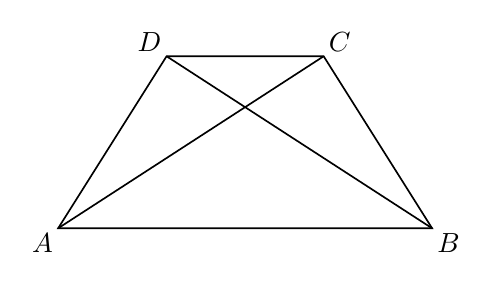
\begin{tikzpicture}[scale=0.95, semithick, every node/.style={inner sep=1.6pt}]
  \coordinate (A) at (0,0);
  \coordinate (B) at (5,0);
  \coordinate (C) at (3.55,2.3);
  \coordinate (D) at (1.45,2.3);

  \draw (A) -- (B) -- (C) -- (D) -- cycle;
  \draw (A) -- (C);
  \draw (B) -- (D);

  \node[below left] at (A) {$A$};
  \node[below right] at (B) {$B$};
  \node[above right] at (C) {$C$};
  \node[above left] at (D) {$D$};
\end{tikzpicture}
\end{center}
\nopagebreak[4]
【B】求矩阵 $\boldsymbol A=\begin{bmatrix}3&2\\2&1\end{bmatrix}$ 的逆矩阵。

【C】已知曲线 $C$ 的参数方程为 $\begin{cases}x=\sqrt t-\dfrac1{\sqrt t},\\ y=3\left(t+\dfrac1t\right),\end{cases}$（$t$ 为参数，$t>0$），求曲线 $C$ 的普通方程。

【D】设 $a\geqslant b>0$，求证：$3a^3+2b^3\geqslant3a^2b+2ab^2$。

\Needspace{4\baselineskip}
\textbf{解析}

\Needspace{5\baselineskip}
【A】由 $\triangle ABC\cong\triangle BAD$（对应 $A\leftrightarrow B$，$B\leftrightarrow A$，$C\leftrightarrow D$）得

\nopagebreak[4]
\[\angle ABC=\angle BAD,\qquad \angle ACB=\angle BDA,\qquad BC=AD .\]

由 $\angle ACB=\angle BDA$ 知 $C$、$D$ 对线段 $AB$ 张等角且在同侧，故 $A$、$B$、$C$、$D$ 四点共圆。

\Needspace{5\baselineskip}
在圆内接四边形 $ABCD$ 中，对角互补：

\nopagebreak[4]
\[\angle BAD+\angle BCD=180^\circ .\]

\Needspace{5\baselineskip}
又 $\angle ABC=\angle BAD$，代入得

\nopagebreak[4]
\[\angle ABC+\angle BCD=180^\circ .\]

这两个角是直线 $AB$、$CD$ 被 $BC$ 所截的同旁内角，故 $AB\parallel CD$。

\Needspace{5\baselineskip}
【B】$|\boldsymbol A|=3\times1-2\times2=-1\neq0$，故 $\boldsymbol A$ 可逆。二阶矩阵的求逆公式为

\nopagebreak[4]
\[\begin{bmatrix}a&b\\c&d\end{bmatrix}^{-1}=\frac1{ad-bc}\begin{bmatrix}d&-b\\-c&a\end{bmatrix},\]

\Needspace{5\baselineskip}
取 $a=3$，$b=2$，$c=2$，$d=1$，得

\nopagebreak[4]
\[\boldsymbol A^{-1}=\frac1{-1}\begin{bmatrix}1&-2\\-2&3\end{bmatrix}=\begin{bmatrix}-1&2\\2&-3\end{bmatrix} .\]

验证：$\begin{bmatrix}3&2\\2&1\end{bmatrix}\begin{bmatrix}-1&2\\2&-3\end{bmatrix}=\begin{bmatrix}1&0\\0&1\end{bmatrix}$。

\Needspace{5\baselineskip}
【C】由 $x=\sqrt t-\dfrac1{\sqrt t}$ 平方得

\nopagebreak[4]
\[x^2=t-2+\frac1t\ \Longrightarrow\ t+\frac1t=x^2+2 .\]

\Needspace{5\baselineskip}
代入 $y=3\left(t+\dfrac1t\right)$ 得

\nopagebreak[4]
\[y=3(x^2+2)=3x^2+6 .\]

\Needspace{5\baselineskip}
当 $t$ 取遍全体正数时，$\sqrt t-\dfrac1{\sqrt t}$ 取遍全体实数，故普通方程为

\nopagebreak[4]
\[y=3x^2+6\quad(x\in\mathbf R).\]

\Needspace{5\baselineskip}
【D】作差：

\nopagebreak[4]
\[3a^3+2b^3-3a^2b-2ab^2=3a^2(a-b)-2b^2(a-b)=(a-b)(3a^2-2b^2) .\]

\Needspace{5\baselineskip}
由 $a\geqslant b>0$ 得 $a-b\geqslant0$，且

\nopagebreak[4]
\[3a^2-2b^2\geqslant3b^2-2b^2=b^2>0 .\]

\Needspace{5\baselineskip}
故 $(a-b)(3a^2-2b^2)\geqslant0$，即

\nopagebreak[4]
\[3a^3+2b^3\geqslant3a^2b+2ab^2 .\]

\gkanswer{答案：A 证明见解析；B $\begin{bmatrix}-1&2\\2&-3\end{bmatrix}$；C $y=3x^2+6$（$x\in\mathbf R$）；D 证明见解析。}

\end{answer}
\begin{answer}
\gksolhead{22}{}

\textbf{题目}：

在平面直角坐标系 $xOy$ 中，抛物线 $C$ 的顶点在原点，经过点 $A(2,2)$，其焦点 $F$ 在 $x$ 轴上。

（1）求抛物线 $C$ 的标准方程；

（2）求过点 $F$，且与直线 $OA$ 垂直的直线的方程；

（3）设过点 $M(m,0)$（$m>0$）的直线交抛物线 $C$ 于 $D$、$E$ 两点，$ME=2DM$，记 $D$ 和 $E$ 两点间的距离为 $f(m)$，求 $f(m)$ 关于 $m$ 的表达式。
\nopagebreak[4]
\begin{center}% 2009 年江苏卷第 22 题：抛物线 y²=2x 与点 A(2,2)、直线 OA。
% 来源 PDF：普通高考/2009/2009江苏.pdf
% SHA-256：64e417d45911d88d77c047a419dcc259e7c7dc779c79d20df2092755c96a4501
% 原页：2009江苏.pdf 第 2 页（A3 三栏）第 3 栏，书页码 532。
% 绘制依据：按原页画坐标轴、抛物线两支、点 A 及线段 OA，并在两轴标出单位刻度 1。
\begin{tikzpicture}[x=0.95cm, y=0.95cm, semithick, every node/.style={inner sep=1.6pt}]
  \draw[->,>=stealth] (-0.7,0) -- (5.6,0) node[below] {$x$};
  \draw[->,>=stealth] (0,-3.4) -- (0,3.5) node[right] {$y$};

  \draw[domain=-3.15:3.15, samples=140, smooth, variable=\t]
    plot ({\t*\t/2}, \t);

  \draw (0,0) -- (2,2);
  \fill (2,2) circle (2.2pt);
  \node[above right] at (2,2) {$A$};

  \draw (1,0) ++(0,-0.09) -- ++(0,0.18);
  \draw (0,1) ++(-0.09,0) -- ++(0.18,0);
  \node[below] at (1,0) {$1$};
  \node[left] at (0,1) {$1$};
  \node[below left] at (0,0) {$O$};
\end{tikzpicture}
\end{center}
\nopagebreak[4]
\Needspace{4\baselineskip}
\textbf{解析}

\Needspace{5\baselineskip}
（1）顶点在原点、焦点在 $x$ 轴上的抛物线可设为 $y^2=2px$（$p>0$）。代入 $A(2,2)$：

\nopagebreak[4]
\[4=2p\times2\ \Longrightarrow\ p=1 .\]

故 $C$ 的标准方程为 $y^2=2x$。

\Needspace{5\baselineskip}
（2）焦点 $F\left(\dfrac12,0\right)$。直线 $OA$ 的斜率为 $\dfrac{2-0}{2-0}=1$，故与 $OA$ 垂直的直线斜率为 $-1$：

\nopagebreak[4]
\[y=-\left(x-\frac12\right),\]

即 $2x+2y-1=0$。

\Needspace{5\baselineskip}
（3）设过 $M(m,0)$ 的直线为 $y=k(x-m)$，代入 $y^2=2x$：

\nopagebreak[4]
\[k^2(x-m)^2=2x\ \Longrightarrow\ k^2x^2-(2k^2m+2)x+k^2m^2=0 .\]

\Needspace{5\baselineskip}
设 $D(x_1,y_1)$、$E(x_2,y_2)$，则

\nopagebreak[4]
\[x_1x_2=m^2 .\]

由 $M$、$D$、$E$ 共线且 $ME=2DM$，得 $|x_2-m|=2|x_1-m|$。结合 $x_1x_2=m^2$，解得 $x_1=\dfrac m2$，$x_2=2m$（另一解 $x_1=x_2=m$ 为退化情形，舍去）。

于是 $y_1^2=2\cdot\dfrac m2=m$，$y_2^2=2\cdot2m=4m$。

\Needspace{5\baselineskip}
又 $D$、$E$ 在 $M$ 两侧，故 $y_2=-2y_1$。于是

\nopagebreak[4]
\[f(m)=|DE|=\sqrt{(x_2-x_1)^2+(y_2-y_1)^2}=\sqrt{\left(\frac{3m}2\right)^2+9m}=\frac32\sqrt{m^2+4m}\quad(m>0).\]

\gkanswer{答案：（1）$y^2=2x$；（2）$2x+2y-1=0$；（3）$f(m)=\dfrac32\sqrt{m^2+4m}$（$m>0$）。}

\end{answer}
\begin{answer}
\gksolhead{23}{}

\textbf{题目}：

对于正整数 $n\geqslant2$，用 $T_n$ 表示关于 $x$ 的一元二次方程 $x^2+2ax+b=0$ 有实数根的有序数组 $(a,b)$ 的组数，其中 $a,b\in\{1,2,\cdots,n\}$（$a$ 和 $b$ 可以相等）；对于随机选取的 $a,b\in\{1,2,\cdots,n\}$（$a$ 和 $b$ 可以相等），记 $P_n$ 为关于 $x$ 的一元二次方程 $x^2+2ax+b=0$ 有实数根的概率。

（1）求 $T_{n^2}$ 和 $P_{n^2}$；

（2）求证：对任意正整数 $n\geqslant2$，有 $P_n>1-\dfrac1{\sqrt n}$。

\Needspace{4\baselineskip}
\textbf{解析}

\Needspace{5\baselineskip}
（1）方程 $x^2+2ax+b=0$ 有实根当且仅当

\nopagebreak[4]
\[\Delta=4a^2-4b\geqslant0\ \Longleftrightarrow\ b\leqslant a^2 .\]

\Needspace{5\baselineskip}
当 $a$ 取 $1,2,\cdots,n^2$ 时，满足条件的 $b\in\{1,2,\cdots,n^2\}$ 有 $\min(n^2,a^2)$ 个。当 $1\leqslant a\leqslant n$ 时 $a^2\leqslant n^2$；当 $n<a\leqslant n^2$ 时 $a^2>n^2$，故

\nopagebreak[4]
\[T_{n^2}=\sum_{a=1}^{n}a^2+\sum_{a=n+1}^{n^2}n^2=\frac{n(n+1)(2n+1)}6+n^2(n^2-n).\]

\Needspace{5\baselineskip}
样本总数为 $(n^2)^2=n^4$，故

\nopagebreak[4]
\[P_{n^2}=\frac{T_{n^2}}{n^4}=\frac{(n+1)(2n+1)}{6n^3}+1-\frac1n=1-\frac1n+\frac{2n^2+3n+1}{6n^3}.\]

（2）记 $k=\lfloor\sqrt n\rfloor$，则 $k^2\leqslant n<(k+1)^2$。

\Needspace{5\baselineskip}
当 $a>k$ 时 $a\geqslant k+1>\sqrt n$，故 $a^2>n$，此时满足 $b\leqslant a^2$ 的 $b$ 有 $n$ 个。这样的 $a$ 有 $n-k$ 个，故

\nopagebreak[4]
\[T_n\geqslant n(n-k).\]

\Needspace{5\baselineskip}
若 $n$ 不是完全平方数，则 $k<\sqrt n$，于是

\nopagebreak[4]
\[P_n=\frac{T_n}{n^2}\geqslant\frac{n-k}{n}=1-\frac kn>1-\frac1{\sqrt n}.\]

\Needspace{5\baselineskip}
若 $n=k^2$，则 $a=k$ 时 $a^2=n$，满足条件的 $b$ 也有 $n$ 个（$b=1,\cdots,n$），故 $a=k,k+1,\cdots,n$ 共 $n-k+1$ 个都贡献 $n$，从而

\nopagebreak[4]
\[T_n\geqslant n(n-k+1),\]

\nopagebreak[4]
\[P_n\geqslant1-\frac{k-1}{n}=1-\frac1{\sqrt n}+\frac1n>1-\frac1{\sqrt n}.\]

综上，对任意正整数 $n\geqslant2$，都有 $P_n>1-\dfrac1{\sqrt n}$。

\gkanswer{答案：（1）$T_{n^2}=\dfrac{n(n+1)(2n+1)}6+n^2(n^2-n)$，$P_{n^2}=1-\dfrac1n+\dfrac{2n^2+3n+1}{6n^3}$；（2）证明见解析。}

\end{answer}